\documentclass[10pt,aspectratio=1610]{beamer}

% -------------------- PACKAGES --------------------
\usepackage[utf8]{inputenc}
\usepackage{graphicx}
\usepackage{mathtools}
\usepackage{utopia}
\usetheme{CambridgeUS}
\usecolortheme{dolphin}
\usepackage{pifont}

\usepackage{tikz}
\usetikzlibrary{positioning,shadows}
\usepackage{algorithm2e}

\usepackage{tcolorbox}
\tcbuselibrary{skins}

\usepackage[comma]{natbib}
\usepackage{hyperref}
\setcitestyle{square}

\usepackage{tabularx}

\beamertemplatenavigationsymbolsempty
\usefonttheme{serif}

% -------------------- COLORS --------------------
\definecolor{myNewColorA}{RGB}{10,50,135}
\definecolor{myNewColorB}{RGB}{25,85,154}
\definecolor{myNewColorC}{RGB}{183,195,230}

\setbeamercolor*{palette primary}{bg=myNewColorC}
\setbeamercolor*{palette secondary}{bg=myNewColorB, fg=white}
\setbeamercolor*{palette tertiary}{bg=myNewColorA, fg=white}
\setbeamercolor*{titlelike}{fg=myNewColorA}
\setbeamercolor*{item}{fg=myNewColorA}

% -------------------- REMOVE TOP BAR --------------------
\setbeamertemplate{headline}{}

% -------------------- FOOTER --------------------
\defbeamertemplate*{footline}{projectfoot}
{
  \leavevmode
  \hbox{
  \begin{beamercolorbox}[wd=.55\paperwidth,ht=2.6ex,dp=1ex,center]{title in head/foot}
    \insertshorttitle
  \end{beamercolorbox}
  \begin{beamercolorbox}[wd=.20\paperwidth,ht=2.6ex,dp=1ex,center]{date in head/foot}
    \insertshortdate
  \end{beamercolorbox}
  \begin{beamercolorbox}[wd=.25\paperwidth,ht=2.6ex,dp=1ex,right]{date in head/foot}
    \insertframenumber{} / \inserttotalframenumber\hspace{0.8em}
  \end{beamercolorbox}}
}
\setbeamertemplate{footline}[projectfoot]

% -------------------- TITLE BLOCK --------------------
\newtcolorbox{titleblock}{
  enhanced,
  colback=myNewColorA,
  colframe=myNewColorA,
  arc=4mm,
  boxrule=0pt,
  left=14pt,
  right=14pt,
  top=12pt,
  bottom=12pt,
  drop shadow={shadow xshift=2mm, shadow yshift=-2mm, fill=black!35}
}

% -------------------- METADATA --------------------
\title[Hybrid KG-RAG]
{Hybrid Knowledge-Graph-Enhanced\\
Retrieval-Augmented Generation for Academic\\
Information Systems}

\subtitle[Final Review]{Final Review}

\author[Group Members]{
\textbf{Group Members}\\[0.3cm]
\begin{tabular}{l}
Julia Mariam John (B23CS2137)\\
Nirmel B Joseph (B23CS2148)\\
Rohith NS (B23CS2156)\\
\end{tabular}\\[0.3cm]
\textbf{Project Guide:} Mr. Praveen J. S.\\
Assistant Professor, Dept. of CSE, MBCET
}

\date[April 2026]{April 2026}

% -------------------- DOCUMENT --------------------
\begin{document}

% 1. Title Slide
\begin{frame}[plain]
\begin{center}
\begin{titleblock}
{\Large\color{white}\bfseries\inserttitle}\\[0.3cm]
{\normalsize\color{white}\insertsubtitle}
\end{titleblock}
\end{center}

\vspace{0.5cm}

\begin{center}
{\normalsize\insertauthor}
\end{center}

\vfill

\begin{center}

\includegraphics[height=2.8cm]{Images/mbcet.png}
\end{center}

\end{frame}

% Contents
\begin{frame}{Contents}
\small
\begin{itemize}
\item Introduction and Motivation
\item Literature Survey
\item Gaps Analysed
\item Stakeholder Comments Regarding the Gaps
\item Problem Statement
\item Objective
\item Flow Diagram
\item Methodology
\item System Architecture
\item Phase 1 \& Phase 2 analysis
\item Results and Discussion
\item Accuracy Graphs
\item Future Enhancement
\item Conclusion
\item References
\end{itemize}
\end{frame}

% ================= INTRODUCTION =================
\section{Introduction}
\begin{frame}{Introduction}
\begin{itemize}
\item Growing dependence on online academic information
\item Institutional data scattered across multiple web sources
\item Limited relational reasoning in conventional retrieval systems
\item Need for intelligent, knowledge-driven academic information systems
\end{itemize}
\end{frame}

% ================= LITERATURE REVIEW =================
\section{Literature Review}
\begin{frame}{Literature Review}
\scriptsize
\begin{tabularx}{\textwidth}{|c|X|X|X|X|}
\hline
Sl.No & Title & Methodology & Results & Limitations\\
\hline
1 & Knowledge graph-extended RAG for QA \cite{kg_rag_springer} 
  & KG-guided retrieval + LLM 
  & Improved multi-hop accuracy 
  & Requires structured knowledge graph\\
\hline
2 & RAG for educational applications \cite{rag_edu_elsevier} 
  & Semantic retrieval + LLM 
  & Reduced hallucination 
  & Dependent on retriever quality\\
\hline
\end{tabularx}
\end{frame}

% ================= RESEARCH GAPS =================
\begin{frame}{Research Gaps Identified}
\begin{itemize}
\item Limited use of knowledge graphs in academic RAG systems
\item Lack of hybrid vector-graph retrieval pipelines
\item Insufficient explainability in LLM-based academic QA
\end{itemize}
\end{frame}



% 5. Stakeholder Comments Regarding the Gaps
\section{Stakeholder Comments}
\begin{frame}{Stakeholder Comments Regarding the Gaps}
\begin{itemize}
    \item Common issues include too many clicks and lack of centralized academic information.
    \item Users mainly visit the college website for exam schedules, syllabus, and academic calendar but find navigation complex due to scattered content.
    \item Many users find it difficult to locate cross-referenced information (e.g., matching a course to its teaching faculty across different PDFs).
    \item Most users believe a chatbot interface would help in faster and easier information access for exam-related and department-specific data.
\end{itemize}
\end{frame}

% ================= PROBLEM STATEMENT =================
\begin{frame}{Problem Statement}
To develop a hybrid knowledge-graph-enhanced retrieval-augmented generation system for accurate and explainable academic information access.
\end{frame}

% 7. Objective
\section{Objective}
\begin{frame}{Objectives}
\begin{enumerate}
\item To collect academic data from institutional websites using web scraping techniques. \ding{51} 
\item To convert the collected text data into vector embeddings for semantic search and retrieval. \ding{51}
\item To construct a knowledge graph of academic entities for Mar Baselios College of Engineering and Technology. \ding{51}
\item To implement an intent-aware query router and integrate hybrid retrieval for query answering. \ding{51}
\item To integrate the retrieved context with a large language model for grounded answer generation. \ding{51}
\end{enumerate}
\end{frame}

% 8. Flow Diagram
\section{Workflow Diagram}
\begin{frame}{Workflow Diagram}
\centering
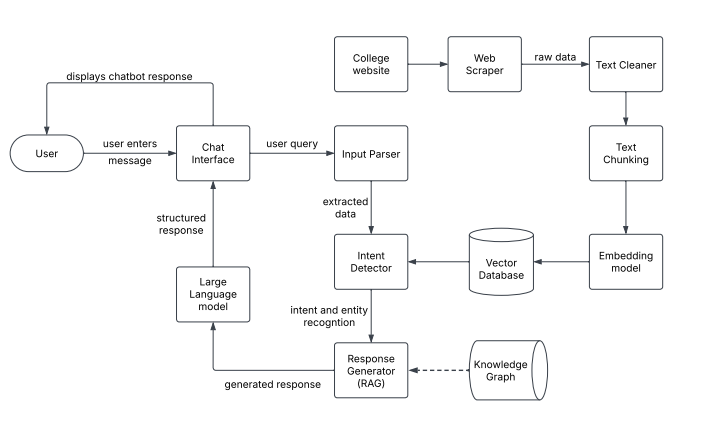
\includegraphics[width=0.9\textwidth]{Images/wf.png}
\end{frame}

% 9. Methodology
\section{Methodology}
\begin{frame}
\frametitle{Methodology}

\begin{itemize}

\item \textbf{Data Collection \& Preprocessing}

HTML pages and PDFs are scraped using BFS URL discovery. The data is parsed, cleaned, and divided into structured semantic chunks preserving hierarchy and entity references.

\item \textbf{Vector Embedding Generation \& Storage}

Each chunk is converted into 768-dimensional embeddings using \textit{EmbeddingGemma} and stored in a \textit{ChromaDB} vector database to capture semantic meaning.

\item \textbf{Knowledge Graph Construction}

A deterministic knowledge graph (JSON) is built connecting Faculty, Course, Program, and Semester entities via strictly evidence-backed edges (\textit{teaches}, \textit{part\_of}).

\end{itemize}

\end{frame}

\begin{frame}
\frametitle{Methodology}

\begin{itemize}

\item \textbf{Intent-Aware Query Routing}

Incoming queries are classified by intent (teaching, faculty, advisory, course, timetable, regulation, general) to dynamically select the optimal retrieval strategy and filtering thresholds.

\item \textbf{Hybrid Retrieval}

The system retrieves the Top-K relevant semantic chunks from the vector database alongside related entity subgraphs from the knowledge graph.

\item \textbf{Answer Generation}

Retrieved information is combined and passed to an LLM, generating accurate, explainable, and context-aware responses constrained to institutional data.

\end{itemize}

\end{frame}

% 10. Architecture / Algorithm
\section{System Architecture}
\begin{frame}{System Architecture}
\centering
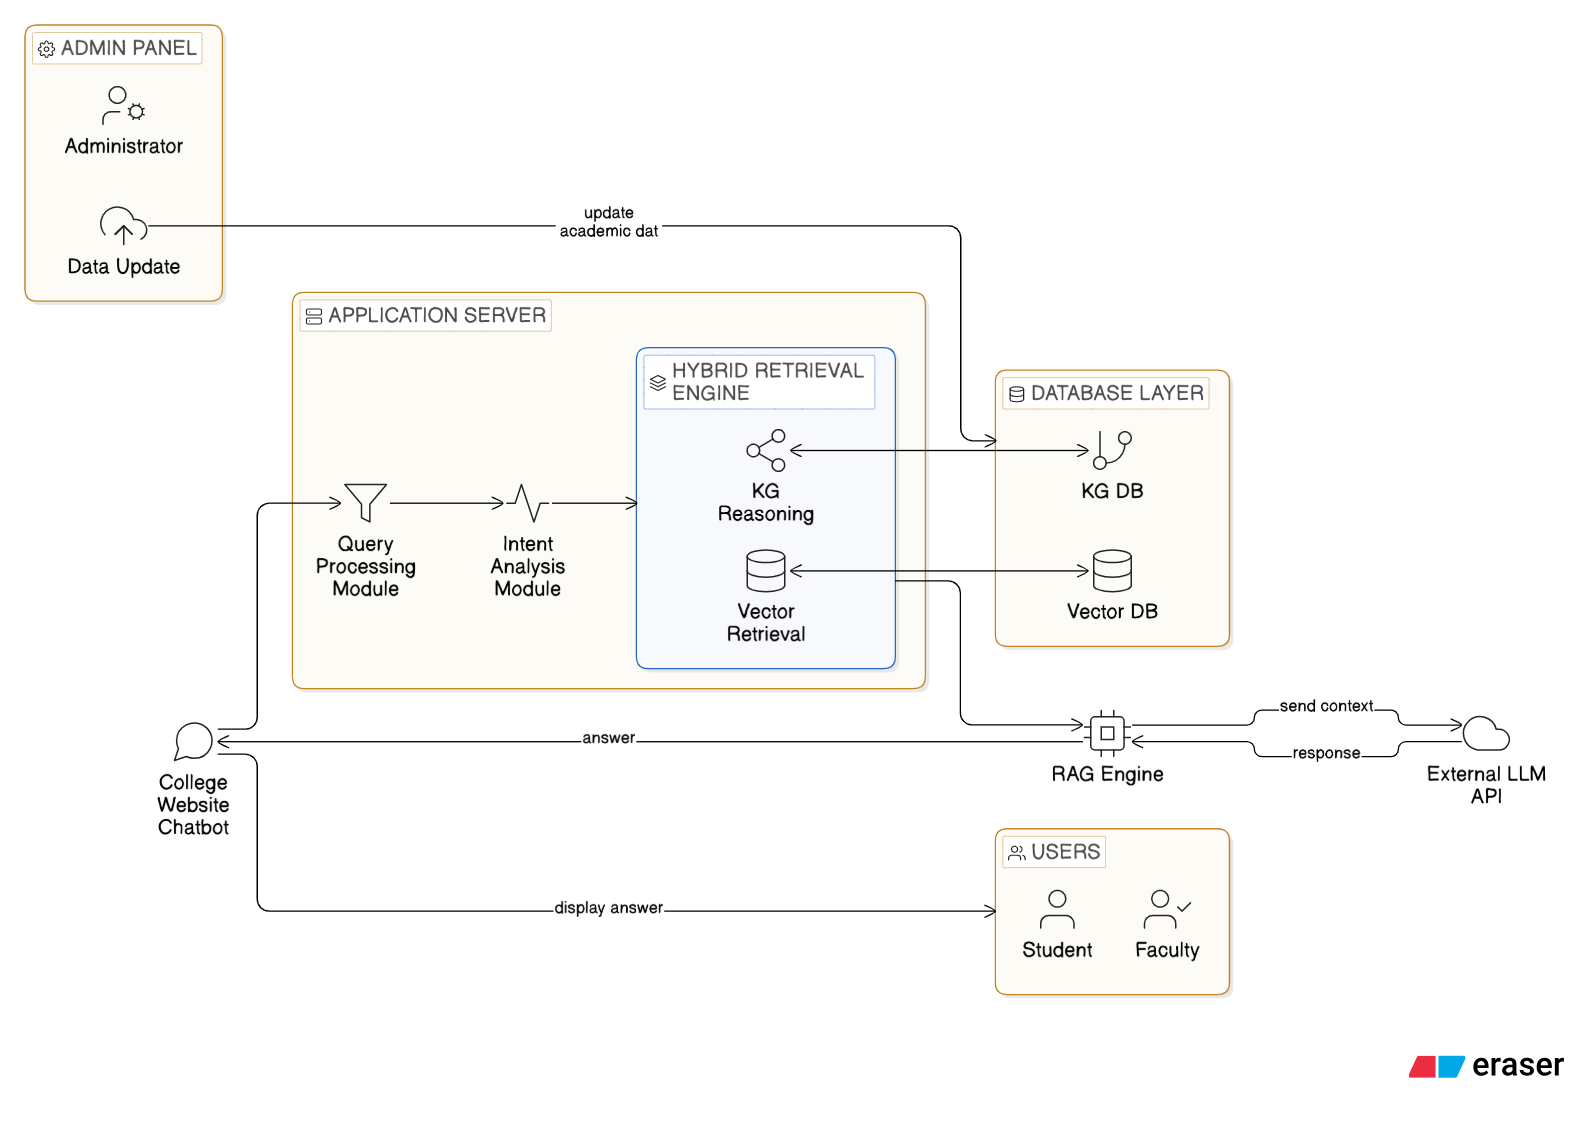
\includegraphics[width=0.88\textwidth]{Images/System Architecture.png}
\end{frame}

% 11. Phase 1 & Phase 2
\section{Experiments / Analysis}
\begin{frame}{Phase 1 \& Phase 2 Analysis}
\textbf{Phase 1: Data Pipeline \& Ingestion}
\begin{itemize}
    \item \textbf{Semantic Chunking:} Generated 2207 chunks (195 HTML, 2012 PDF) spanning tables, profiles, sections, regulations, and lists, with rigorous deduplication.
    \item \textbf{Vector Database:} Ingested 2268 vector documents into ChromaDB.
    \item \textbf{Knowledge Graph:} Constructed a 480-node graph with 1700 deterministic edges, maintaining a metadata completeness ratio of 1.000.
\end{itemize}

\vspace{0.3cm}
\textbf{Phase 2: Hybrid Retrieval Evaluation}
\begin{itemize}
    \item Evaluated over 30 representative queries spanning multi-hop and semantic intents using top-$k=5$.
    \item Tested intent-based routing with adaptive distance thresholding (0.6 for excellent matches, scaling to 0.8 for poor matches).
\end{itemize}
\end{frame}

% 12. Results and Discussion
\section{Results and Discussion}
\begin{frame}{Results and Discussion}
\textbf{Retrieval Quality Metrics}
\begin{itemize}
    \item \textbf{HitRate@5:} 0.767
    \item \textbf{Mean Reciprocal Rank (MRR):} 0.740
    \item \textbf{NDCG@5:} 0.841
    \item \textbf{Precision@5:} 0.600 $\vert$ \textbf{Recall@5:} 0.733
\end{itemize}

\vspace{0.3cm}
\textbf{Discussion}
\begin{itemize}
    \item The system achieved a \textbf{100\% hit rate} on core academic intents (teaching, faculty, course, and timetable).
    \item \textbf{Regulation queries} remained a weakness, often drifting towards table content and triggering robust fallbacks.
    \item The knowledge graph exhibited strong structural coverage with a \textbf{98.3\% largest connected component ratio} and only a 1.7\% orphan ratio.
\end{itemize}
\end{frame}

% 13. Accuracy / Precision Graphs
\section{Workflow Diagram}
\begin{frame}{Accuracy Graph - Retrieval Hit Rate by Query Type}
\centering
\includegraphics[width=0.9\textwidth]{Images/hit.png}
\end{frame}

% 14. Future Enhancement
\section{Future Enhancement}
\begin{frame}{Future Enhancement}
\begin{itemize}
    \item \textbf{Prerequisite Edge Extraction:} Enhance context window disambiguation to populate \textit{has\_prerequisite} edges reliably.
    \item \textbf{Regulation Retrieval Improvement:} Retune route-specific thresholds and implement tighter regulation-aware filtering.
    \item \textbf{Runtime Optimization:} Persist embedding models in memory to avoid per-query initialization delays and reduce system latency.
    \item \textbf{Ecosystem Scaling:} Extend the existing pipeline beyond the CSE department to cover other institutional branches.
\end{itemize}
\end{frame}

% 15. Conclusion
\section{Conclusion}
\begin{frame}{Conclusion}
\begin{itemize}
\item Hybrid KG-RAG dramatically improves academic information retrieval for highly unstructured multi-document environments.
\item Combining semantic embeddings with graph-guided relationship mapping provides accurately grounded answers for complex queries.
\item By systematically classifying user intents and providing explainable responses, the system significantly outperforms keyword-based paradigms.
\item The project successfully addressed the identified domain challenges, closely aligning with SDG~4 and SDG~9.
\end{itemize}
\end{frame}

% 16. References
\section{References}
\begin{frame}{References}
\scriptsize
\bibliographystyle{ieeetr}
\begin{thebibliography}{99}

\bibitem{kg_rag_springer}
J.~Linders and J.~M.~Tomczak,
``Knowledge graph-extended retrieval augmented generation for question answering,''
\emph{Applied Intelligence}, vol.~55, no.~17, pp.~1102--1118, 2025.

\bibitem{rag_edu_elsevier}
Z.~Li et al.,
``Retrieval-augmented generation for educational application: A systematic survey,''
\emph{Computers and Education: Artificial Intelligence}, vol.~8, p.~100417, 2025.

\bibitem{lewis2020}
P.~Lewis et al.,
``Retrieval-augmented generation for knowledge-intensive NLP tasks,''
\emph{NeurIPS}, vol.~33, pp.~9459--9474, 2020.

\bibitem{pan2024}
S.~Pan et al.,
``Unifying large language models and knowledge graphs: A roadmap,''
\emph{IEEE TKDE}, vol.~36, no.~7, pp.~3580--3599, 2024.

\end{thebibliography}
\end{frame}

% Thank You
\begin{frame}
\centering
\Huge \textcolor{myNewColorA}{Thank You}
\end{frame}

\end{document}
